\section{Prüfung 14.04.2021}
\subsection{Echtzeit}
\subsubsection{a)}
Ein Zugführer muss in den ersten 30 Sekunden jeder Minute den Totmannknopf drücken um
anzuzeigen dass er noch am Leben ist. Unterbleibt das rechtzeitige Drücken des Totmannknopfes,
macht der Zug automatisch eine Notbremsung.
Zeichnen Sie in das Diagramm unten den Verlauf der Profit-Penalty-Funktion für die Operation
„Totmannknopf drücken“ über die gesamte Zeitachse hinweg ein.

\begin{figure}[H]
  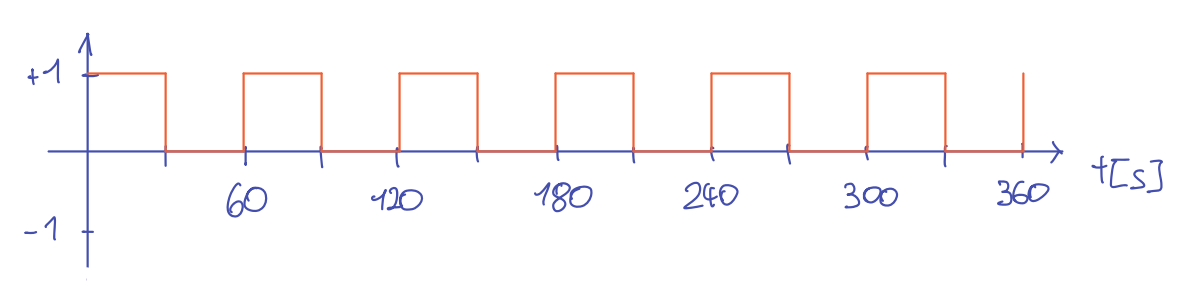
\includegraphics[width=10cm]{images/KA140421/1a.PNG}
  \centering
\end{figure}

\subsubsection{b)}
Es handelt sich um feste Echtzeit. Verpasst der Lokführer den 30s Zeitraum kommt der Zug zum Stehen, der 
Zug wird nicht beschädigt und es wird (wahrscheinlich) auch niemand verletzt.

\subsection{Architektur, Plattformen und Vernetzung}
\subsubsection{a)}
Nennen Sie je einen Vor- und Nachteil eines dreifach redundanten Kontrollsystems gegenüber einem
Standby-Kontrollsystem.

Vorteile:
\begin{itemize}
  \item Hohe Sicherheit
  \item Hohe Robustheit
  \item bessere Fehlererkennung
\end{itemize}

Nachteile:
\begin{itemize}
  \item Hohe Kosten
  \item komplexer
  \item Höhere Latenz
\end{itemize}

\subsubsection{b)}
Nennen Sie mindestens vier Kriterien von denen die Wahl der Plattform (Standardprozessor,
Spezialprozessor, ASIC, FPGA) beim Entwurf eines eingebetteten Echtzeitsystems abhängen sollte.

Kosten, Entwicklungsdauer, Anwendung, Prototyp / Serienprodukt, Flexibilität, Leistungsanforderungen, Effizienz

\subsubsection{c)}
Warum ist Standard-Ethernet nicht echtzeitfähig?

Aufgrund der CSMA/CD Methode und TCP/IP Protokoll ist Ethernet nicht echtzeitfähig.
CSMA/CD (\textbf{C}arrier \textbf{S}ense \textbf{M}ultiple \textbf{A}ccess / \textbf{C}ollision \textbf{D}etection).

\subsubsection{d)}
Nennen Sie mindestens zwei Vorteile die der Einsatz einer Spezifikationssprache beim Entwurf
eingebetteter Echtzeitsysteme bietet.

\begin{itemize}
  \item Verbesserte Übersichtlichkeit und Verständlichkeit, es können Programmieranfänger mit solchen Sprachen umgehen.
  \item Effizientere Entwicklung und Überprüfung
  \item Verringerung von Fehlern und Konflikten
\end{itemize}

\subsection{Echtzeitscheduling}
Die Abbildung zeigt den Schedule für die Ausführung der folgenden präemptiven Tasks T1, T2, T3 auf einem
Prozessor.\\
T1 = (1; 3),\\
T2 = (2; 6),\\
T3 = (4; 12)\\
wobei ein Task als "Tn = (Ausführungszeit; Periode)" definiert ist. Für jeden Task ist die Periode identisch
mit der Deadline. Das Scheduling aller Tasks beginnt gleichzeitig zum Zeitpunkt 0.

\begin{figure}[H]
  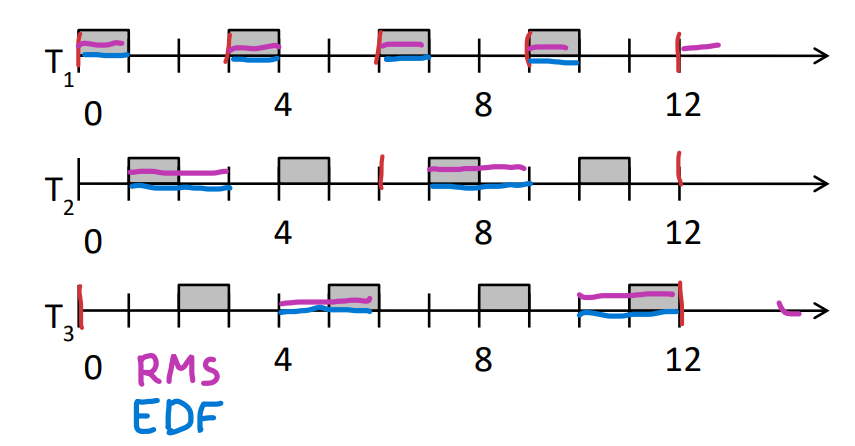
\includegraphics[width=10cm]{images/KA140421/3a.PNG}
  \centering
\end{figure}

\subsubsection{a)}
Werden in der Abbildung alle Deadlines eingehalten? Falls nicht, geben Sie die erste Verletzung
einer Deadline an.

Ja es werden alle Deadlines eingehalten.

\subsubsection{b)}
Wurde dieses abgebildete Schedule mit EDF erzeugt? Begründen Sie.

Nein, der Schedule wurde mit Round Robin erzeugt.

\subsubsection{c)}
Wurde dieses abgebildete Schedule mit RMS erzeugt? Begründen Sie.

Nein, der Schedule wurde mit Round Robin erzeugt.

\subsection{Tasksynchronisation}
Gegeben seien wie unten gezeigt zwei periodische Tasks T1 und T2, die auf die gemeinsame Variable X
zugreifen. Zu Beginn hat X den Wert 2. Gehen Sie ferner davon aus, dass der Scheduler immer den
ausführbereiten Task mit der höchsten Priorität ausführt. Wenn mehrere ausführbereite Tasks die gleiche
höchste Priorität haben wird gemäß Round-Robin mit Zeitscheiben und Verdrängung (Preemption)
ausgeführt.

\begin{figure}[H]
  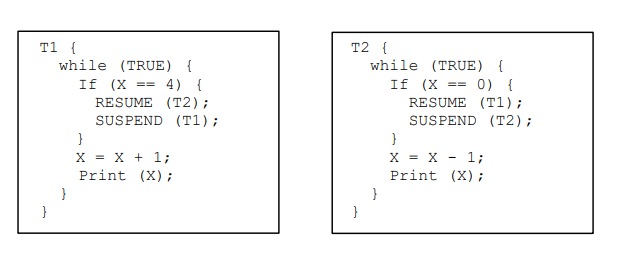
\includegraphics[width=10cm]{images/KA140421/4a.PNG}
  \centering
\end{figure}

\subsubsection{a)}
Welche Ausgabefolge wird generiert falls T1 eine höhere Priorität als T2 hat?

3, 4, 3, 2, 1, 0, 1, 2, 3, 4, 3, 2, 1,\dots

\subsubsection{b)}
Die Zeile $X = X + 1$ besteht aus einer Lese und einer darauf folgenden Schreiboperation.
z.B. $X=1$. Liest T1 X aus merkt er sich $X=1$, jetzt wird T2 gescheduled und T2 liest und erniedrigt X auf $X=0$.
Wird jetzt wieder T1 gescheduled denkt T1 immer noch, dass $X=1$ ist und erhöht X auf $X=2$. Es kommt zu einem
fehlerhaften Verhalten.

\subsection{Spezifikationssprachen}
Zeichnen Sie einen StateChart für die Steuerung eines Verkaufsautomaten welcher 50 Cent und 1 EUR
Münzen akzeptiert und eine Manner-Schnitte für 2 Euro verkauft. Wenn der Benutzer innerhalb von 30
Sekunden genau 2 Euro einwirft wird die Manner-Schnitte ausgegeben, sonst wird das Geld wieder
ausgegeben. Danach begibt sich der Automat wieder in den Ausgangszustand und ist bereit für den
nächsten Kunden. Eingabeereignisse sind das Einwerfen der beiden Münzen, die Ausgaben sind MANNER
und GELDZURUECK.
Geben Sie wie bei Statecharts üblich die Namen aller Zustände an, markieren Sie Transitionen mit Eingaben
bzw. Ereignissen und Ausgaben, geben Sie die Startzustände an.

ka...
\subsection{Speicherprogrammierbare Steuerung (SPS)}
In folgender Ablaufsteuerung werden drei Boolesche Variablen A, B und C verwendet die zu Beginn alle den
Wert FALSE haben. 

\begin{figure}[H]
  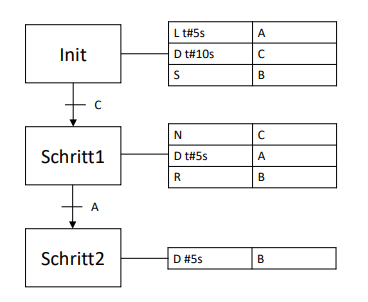
\includegraphics[width=10cm]{images/KA140421/6a.PNG}
  \centering
\end{figure}

Geben Sie für jede Variable eine Folge von Zeitintervallen an wann diese Variable den Wert TRUE hat. Für
jede Variable kann es mehrere solche Intervalle geben. Zum Beispiel bedeutet [3, 4] dass eine Variable von
3 Sekunden nach Beginn der Ausführung bis 4 Sekunden nach Beginn der Ausführung den Wert TRUE hat.

A: [0 ,5 ] [15,15] [/,/ ]\\
B: [0 ,10] [/ ,/ ] [20,-]\\
C: [10,10] [10,15] [/,/ ]

\begin{figure}[H]
  \includegraphics[width=8cm]{images/KA140421/6_erklärung.PNG}
  \centering
\end{figure}

\begin{figure}[H]
  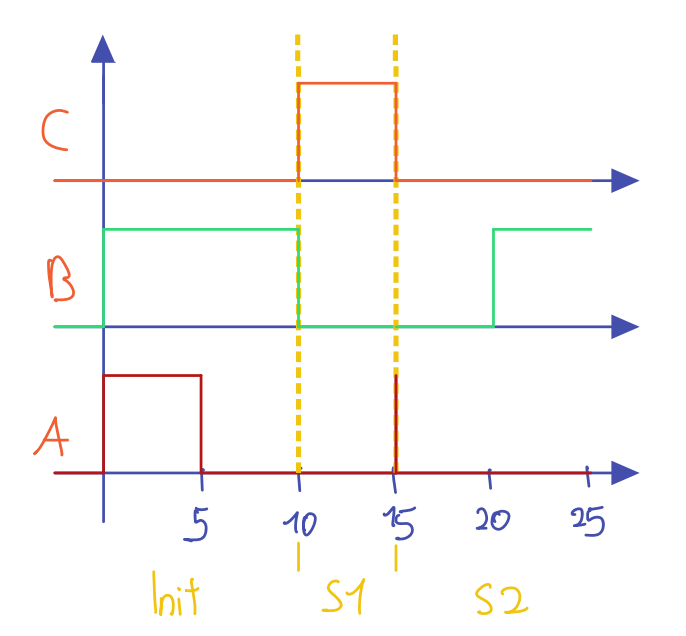
\includegraphics[width=8cm]{images/KA140421/6a_2.PNG}
  \centering
\end{figure}